\chapter{\label{ch:4-accel}Dependence Graph Model for FMU Co-simulation} 

\minitoc

This chapter describes a dependence graph model that is used in this thesis for representing a co-simulation program. The different phases for building the said model are explained including the initial construction of the dependence graph, transformations that it undergoes in order to represent multi-rate co-simulation and mutual exclusion constraints, and finally rules for characterizing the graph with real-time parameters.
 
\section{\label{sec:4-depgrph}Dependence Graph of an FMU Co-simulation}

Automatic parallelization of computer programs embodies the adaptation of the potential parallelism inherent in the program to the effective parallelism that is provided by the hardware. Because computer programs are usually complex, this process of adaptation requires the use of a model for abstracting the program to be parallelized. The aim of using such model is to identify which parts of the program can be executed in parallel. The model has also to represent other features of the program such as data dependence between different pieces of the code. Task dependence graphs are commonly used for this purpose. A task dependence graph is a DAG denoted $G(V,A)$ where:
\begin{itemize}
\item $V$ is the set of vertices of the graph. The size of the graph $n$ is equal to the number of its vertices. Each vertex $v_i: 0 \leq i < n$ represents a task which is an atomic unit of computation.
\item $A$ is the set of arcs of the graph. An arc is denoted as a pair $(v_i,v_j)$ and describes a precedence constraint between $v_i$ and $v_j$, i.e. $v_i$ has to finish its execution before $v_j$ can start its execution. $v_i$ is called the \textit{head} vertex and $v_j$ is called the \textit{tail} vertex. 
\end{itemize}

In the remainder of the thesis, we shall use the term dependence graph instead of task dependence graph.

The dependence graph defines the partial order to be respected when executing the set of tasks. This partial order describes the potential parallelism of the program. %Figure \ref{} shows an example of a task dependence graph of size $5$.

The co-simulation of FMUs lends itself to the dependence graph representation as shown hereafter. According to the FMI standard, the code of an FMU can be exported in the form of source code or as precompiled binaries. However, most FMU providers tend to adopt the latter option for proprietary reasons. We are thus interested in this case. The method for automatic parallelization of FMU co-simulation that we propose in this thesis is based on representing the co-simulation as a dependence graph. We present in the rest of this section how this graph is constructed and a set of attributes that characterize it. The graph construction and characterization method is part of the RCOSIM approach as presented in \cite{benkhaled:2014}.

\subsection{Construction of the Dependence Graph of an FMU Co-Simulation}

The entry point for the construction of a dependence graph of an FMU co-simulation is a user-specified set of interconnected FMUs as depicted in Figure~\ref{fig:2mdlsbb}. The execution of each FMU is seen as computing a set of input operations (one operation for each of the inputs of the FMU), a set of output operations (one operation for each of the outputs of the FMU), and one state operation for updating the state variables of the FMU. An operation is defined by a number of FMU C function calls. An input (resp. output ) operation is executed by calling \textit{fmiSet} (resp. \textit{fmiGet}) function and a state operation is executed by calling \textit{SetTime, GetDerivatives, SetContinuousStates, etc.}, functions in the case of FMI for Model Exchange or \textit{DoStep} function in the case of FMI for Co-Simulation. Thanks to FMI, it is additionally possible to access information about the internal structure of a model encapsulated in an FMU. In particular, as shown in Figure~\ref{fig:2mdlsintra}, FMI allows the identification of Direct Feedthrough (e.g. $Y_{B1}$) and Non Direct Feedthrough (e.g. $Y_{A1}$) outputs of an FMU and other information depending on the version of the standard:

\begin{itemize}
\item FMI 1.0: Dependencies between input operations and output operations are given. The computation of the state at a given simulation step $k$ is considered necessary for the computation of each one of the output operations at the same simulation step $k$. It is considered that the computation of the state at a simulation step $k+1$ requires the computation of each of the input operations at the simulation step $k$.
\item FMI 2.0: In addition to the information provided in FMI 1.0, more information is given about data dependencies. It is specified which output operations at a given simulation step depend on the state computation at the same step. Also, it is specified which input operations at a simulation step $k$ need to be computed before the computation of the state at the step $k+1$.  
\end{itemize}

\begin{figure}[htb]
\centering
\begin{subfigure}{.5\textwidth}
  \centering
  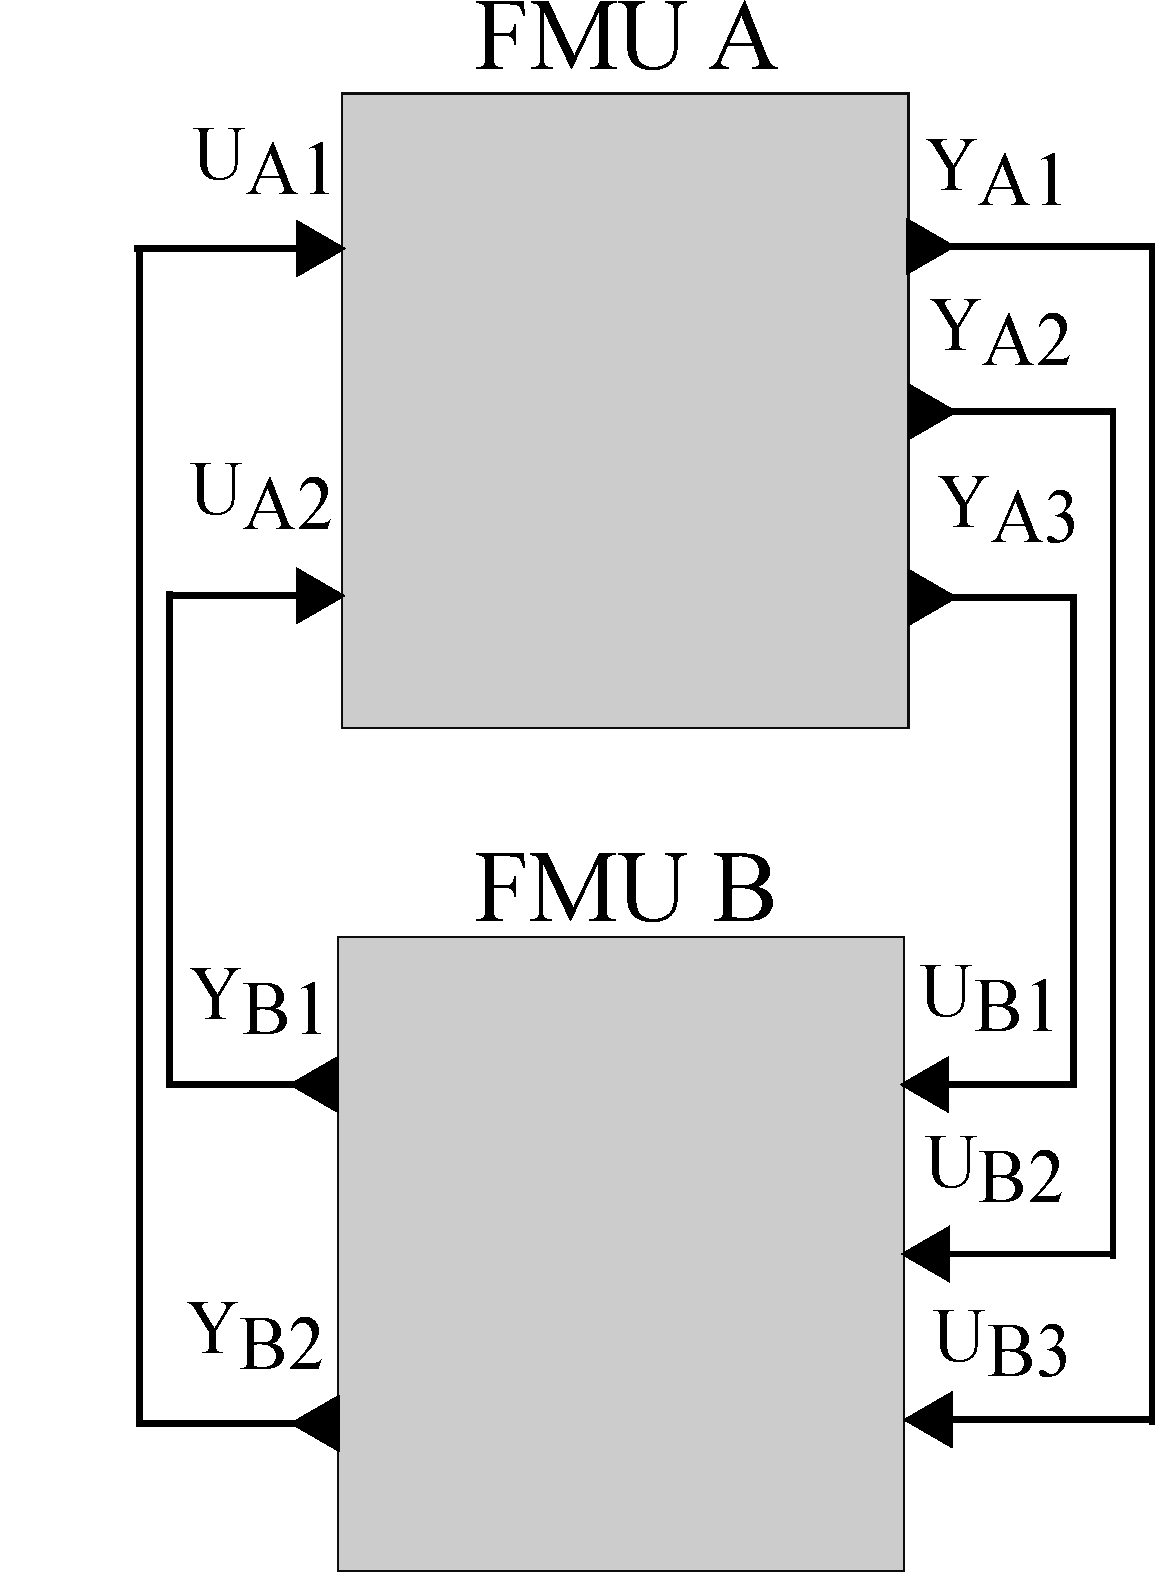
\includegraphics[scale=0.2]{figures/Two_Models_Black_Box}
  \caption{Inter-FMU dependencies specified by the user}
  \label{fig:2mdlsbb}
\end{subfigure}%
\begin{subfigure}{.5\textwidth}
  \centering
  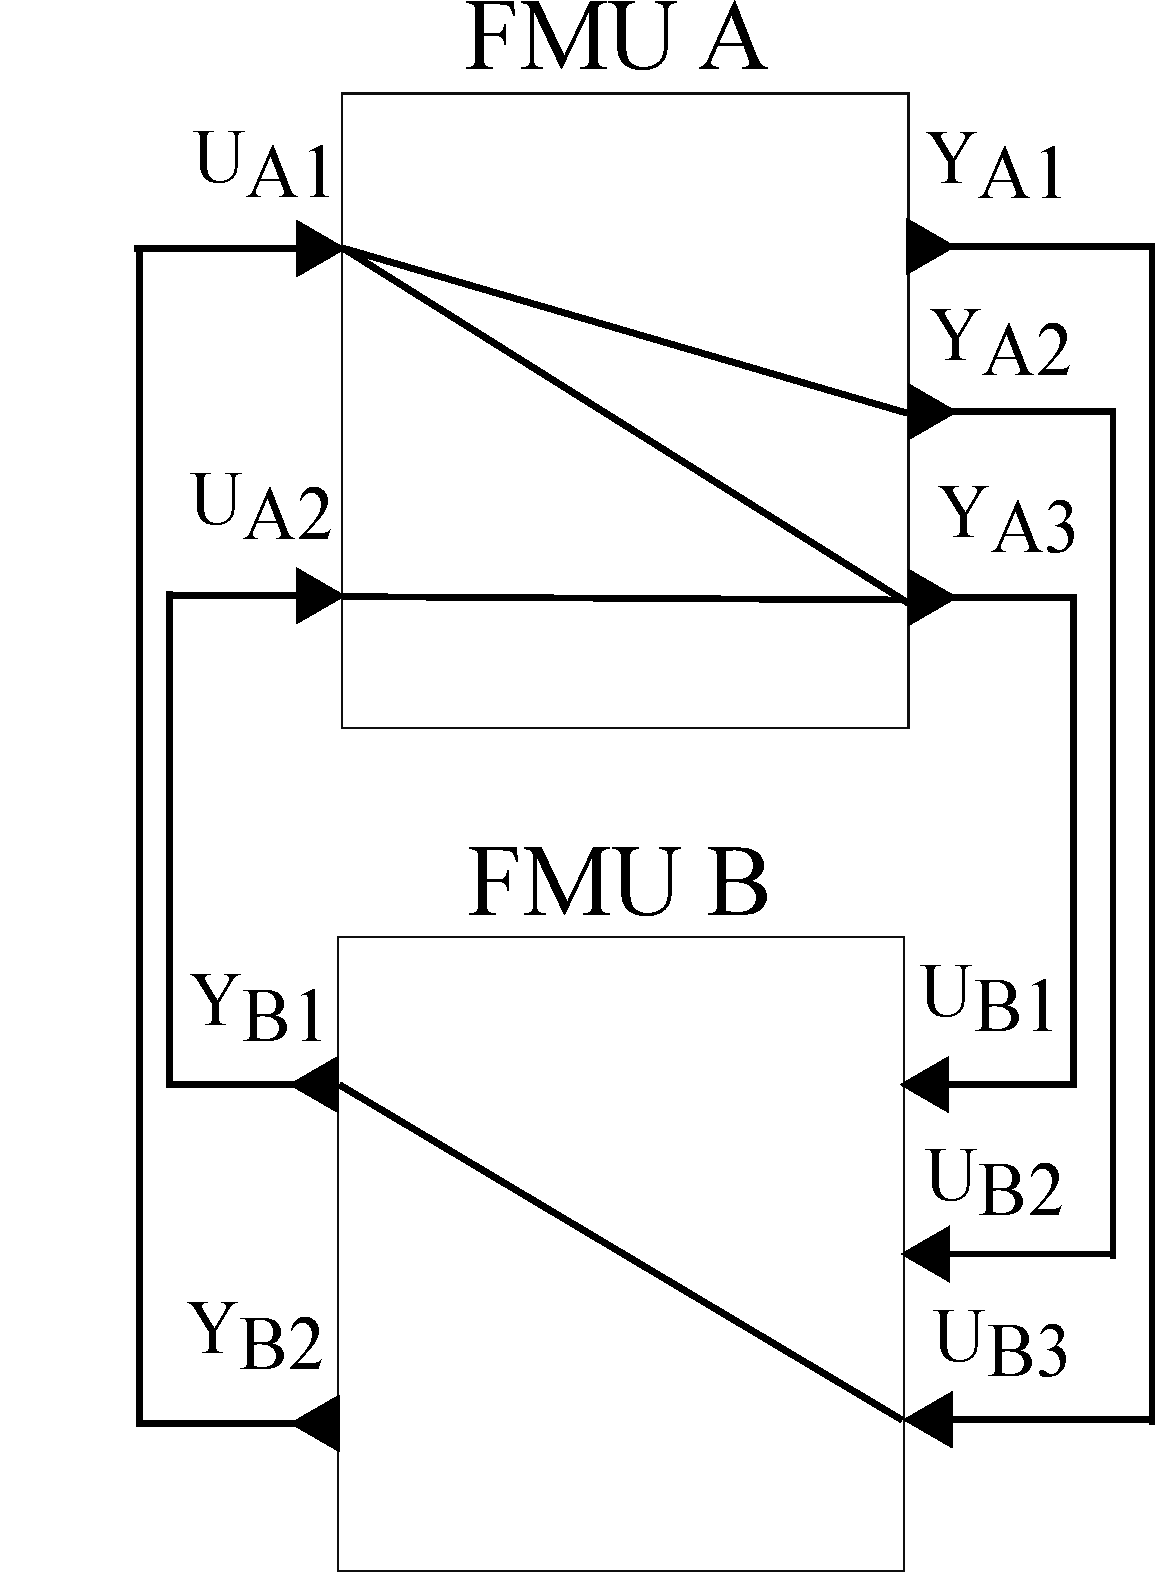
\includegraphics[scale=0.2]{figures/Two_Models}
  \caption{Intra-FMU dependencies provided by FMI}
  \label{fig:2mdlsintra}
\end{subfigure}
\caption{An example of inter and intra-FMU dependencies of two FMUs connected by the user}
\label{fig:2mdls}
\end{figure}

FMU information on input/output dependencies allows building a graph with an increased granularity. The co-simulation is described by a dependence graph $G(V,A)$ called the operation graph where each vertex $o_i \in V: 0 \leq i < n$ represents one operation, each arc $(o_i,o_j) \in A: 0 \leq i,j < n$ represents a precedence relation between operations $o_i$ and $o_j$, and $n = |V|$ is the size of the operation graph. The operation graph is built by exploring the relations between the FMUs and between the operations of the same FMU. A vertex is created for each operation and arcs are then added between vertices if a precedence dependence exists between the corresponding operations. If FMI 1.0, which does not give information about the dependencies between the state variables computation and the input and output variables computations, is used, we must add arcs between all input operations and the state operation of the same FMU. Furthermore, arcs connect all output operations and the state operation of the same FMU because the computation at the simulation step $k$ of an output must be performed with the same value of the state (computed at simulation step $k$) as for all the outputs belonging to the same FMU. Running the co-simulation consists in executing the graph repeatedly. A new execution of the graph cannot be started unless the previous one was totally finished. The operation graph corresponding to the FMUs of Figure~\ref{fig:2mdls} is shown in Figure~\ref{fig:dag}.

\begin{figure}[htb]
\centering
  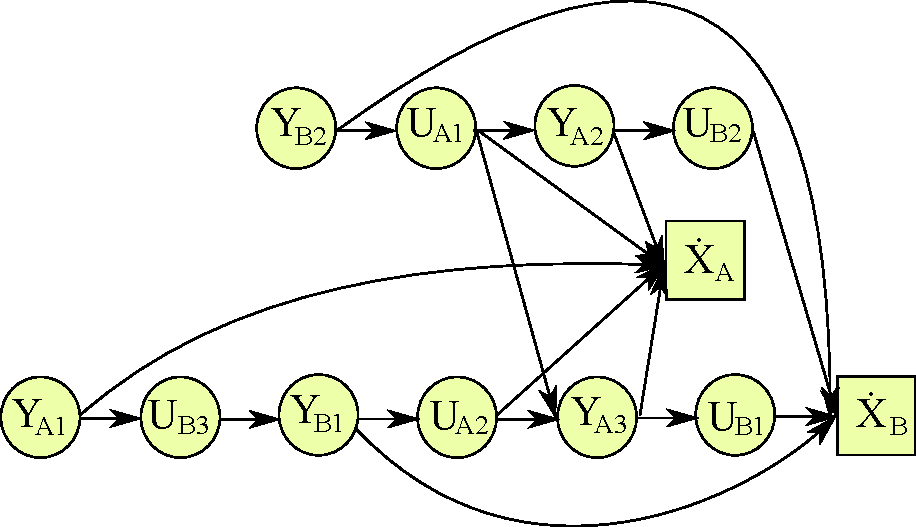
\includegraphics[scale=0.5]{figures/Operation_Graph_Two_Models}
\caption{Operation graph obtained from the FMUs of Figure~\ref{fig:2mdls}}
\label{fig:dag}
\end{figure} 

\subsection{Dependence Graph Attributes}

The dependence graph is used as input to the scheduling algorithm. In addition to the structure of the graph, the scheduling algorithm uses a number of attributes to compute an efficient schedule of the dependence graph. Many list scheduling algorithms use attributes that are computed by the Critical Path Method. We define a set of attributes and notations to characterize the FMU dependence graph.

The notation $f_m(o_i)$ is used to refer to the FMU to which the operation $o_i$ belongs, and $T(o_i)$ to denote the type of the operation $o_i$, i.e. $T(o_i) \in \{update_{input}, update_{output}, update_{state}\}$. $o_j$ is a predecessor of $o_i$ if there is an arc from $o_j$ to $o_i$, i.e. $(o_j, o_i) \in A$. We denote the set of predecessors of $o_i$ by $pred(o_i)$. $o_j$ is an ancestor of $o_i$ if there is a path in $G$ from $o_j$ to $o_i$. The set of ancestors of $o_i$ is denoted by $ance(o_i)$. $o_j$ is a successor of $o_i$ if there is an arc from $o_i$ to $o_j$, i.e. $(o_i, o_j) \in A$. We denote the set of successors of $o_i$ by $succ(o_i)$. $o_j$ is a descendant of $o_i$ if there is a path in $G$ from $o_i$ to $o_j$. The set of descendants of $o_i$ is denoted by $desc(o_i)$. A profiling phase allows measuring the execution time $C(o_i)$. For each operation, the average execution time of multiple co-simulation runs is used. When real-time execution is aimed, Worst Case Execution Times (WCET) are used instead. An operation $o_i$ is characterized by its communication step $H(o_i)$ which is equal to the communication step of its FMU. The earliest start time from start $S(o_i)$ and the earliest end time form start $E(o_i)$ are defined by equations \ref{eq:sfs} and \ref{eq:efs} respectively. $S(o_i)$ defines the earliest time at which the operation $o_i$ can start its execution. $S(o_i)$ is constrained by the precedence relations. The earliest time the operation $o_i$ can finish its execution is defined by $E(o_i)$.

\begin{equation}
S(o_i)=\begin{cases}
    0, & \text{if $pred(o_i)=\emptyset$}.\\
    max_{o_j \in pred(o_i)}(E(o_j)), & \text{otherwise}.
  \end{cases}
	\label{eq:sfs}
\end{equation}

\begin{equation}
	E(o_i)=S(o_i)+C(o_i) 
	\label{eq:efs}
\end{equation}

The latest end time from end $\overline{E}(o_i)$ and the latest start time form end $\overline{S}(o_i)$ are defined by equations \ref{eq:efe} and \ref{eq:sfe} respectively. %$\overline{E}(o_i)$ defines the latest time by which the operation $o_i$ must finish its execution so as not to increase the total execution time of the graph. For $o_i$ to finish its execution no later than $\overline{E}(o_i)$, it has to start its execution at the latest at $\overline{S}(o_i)$. 

\begin{equation}
\overline{E}(o_i)=\begin{cases}
    0, & \text{if $succ(o_i)=\emptyset$}.\\
    max_{o_j \in succ(o_i)}(\overline{S}(o_j)), & \text{otherwise}.
  \end{cases}
	\label{eq:efe}
\end{equation}

\begin{equation}
	\overline{S}(o_i)=\overline{E}(o_i)+C(o_i) 
	\label{eq:sfe}
\end{equation}

The critical path of the graph is the longest path in the graph. The length of a path is computed by accumulating the execution times of the operations that belong to it. The length of the critical path of the graph $R$ is defined by equation \ref{eq:crit}. The critical path is a very important characteristic of the dependence graph. It defines a lower bound on the execution time of the graph, i.e. in the best case the time needed to execute the whole graph is equal to the length of the critical path. 

\begin{equation}
	R = \max_{o_i \in V_I}(E(o_i)) 
	\label{eq:crit}
\end{equation}
 
The flexibility $F(o_i)$ is defined by equation \ref{eq:flex}. $F(o_i)$ expresses the length of an execution interval within which operation $o_i$ can be executed without increasing the total execution time of the graph.

\begin{equation}
	F(o_i) = R - S(o_i) - C(o_i) - \overline{E}(o_i) 
	\label{eq:flex}
\end{equation}

\section{Dependence Graph of a Multi-rate FMU Co-simulation}

The FMU dependence graph model presented in the previous section allows elementary modeling of FMU co-simulation programs. For some applications this model is sufficient to be used for multi-core scheduling. However, many industrial co-simulation applications feature behaviors that cannot be captured by this model. In particular, many industrial applications involve FMUs that are executed according to different communication steps. This is especially true when some FMUs of one co-simulation are provided by different parties. It is very common that an FMU provider designs the FMU in such a way that its proper functioning depends on the use of specific values of the communication step. It is therefore highly unrecommended, and in some cases even impossible, to change the communication step of the FMU. In other cases, even if it is possible and acceptable to change the communication step of a given FMU, better performance and/or accuracy could be obtained when using specific communication steps. As a consequence, our FMU dependence graph model has to be extended in order to accommodate multi-rate data exchange between operations. 

Consider a dependence graph that is constructed as described in the previous section from a multi-rate co-simulation, i.e. some FMUs have different communication steps. Such graph is referred to as a multi-rate dependence graph. One way for making such dependence graph suitable for multi-core scheduling is to transform it into a mono-rate graph. This section presents an algorithm that transforms the initial multi-rate operation graph $G(V,A)$ into a mono-rate operation graph $G_M(V_M,A_M)$. The aim of this transformation is to ensure that each operation is executed according to the communication step of its respective FMU and also to maintain a correct data exchange between the different FMUs, whether they have different or identical communication steps. Similar algorithms have been used in the real-time scheduling literature \cite{kermia:2009, ramamritham:1995}.

We define the \textit{Hyper-Step (HS)} as the least common multiple ($lcm$) of the communication steps of all the operations: $HS=lcm(H(o_1),H(o_2), \dots ,H(o_n))$ where $n = |V_I|$ is the number of operations in the initial graph. The Hyper-Step is the smallest interval of time for describing a repeatable pattern of all the operations. The transformation algorithm consists first of all in repeating each operation $o_i$, $r_i$ times where $r_i$ is called the repetition factor of $o_i$ and $r_i = \frac{HS}{H(o_i)}$. Each repetition of the operation $o_i$ is called an occurrence of $o_i$ and corresponds to the execution of $o_i$ at a certain simulation step. We use a superscript to denote the number of each occurrence, for instance $o_i^s$ denotes the $s^{th}$ occurrence of $o_i$. Then, arcs are added between operations following the rules presented hereafter. Consider two operations $o_i, o_j \in V_I$ connected by an arc $(o_i,o_j) \in A_I$, then adding an arc $(o_i^s,o_j^u)$ to $A_M$, depends on the simulation steps (time) at which $o_i^s$ and $o_j^u$ are executed. In other words, if $k_{s}$ and $k_{u}$ are the simulation steps associated with $o_i^s$ and $o_j^u$ respectively, then the inequality $k_{s} \leq k_{u}$ is a necessary condition to add the arc $(o_i^s,o_j^u)$ to $A_M$. In addition, $o_j^u$ is connected with the latest occurrence of $o_i$ that satisfies this condition, i.e. with the occurrence $o_i^s$ such that $s=\max(0,1, \dots ,r_i-1) : k_{s} \leq k_{u}$. In the case where $H(o_i) = H(o_j)$ (and therefore $r_i = r_j$), occurrences $o_i^s$ and $o_j^u$ which correspond to the same number, i.e. $s = u$, are connected by an arc. On the other hand, if $H(o_i) \neq H(o_j)$, we distinguish between two types of dependencies: we call the arc $(o_i,o_j) \in A_I$ a \textit{slow to fast} (resp. \textit{fast to slow}) dependence if $H(o_i) > H(o_j)$ (resp. $H(o_i) < H(o_j)$). For a slow to fast dependence $(o_i,o_j) \in A_I$, one occurrence of $o_i$ is executed while several occurrences of $o_j$ are executed. In this case, arcs are added between each occurrence $o_i^s: s \in \{0,1, \dots ,r_i-1\}$, and the occurrence $o_j^u$ such that:

\begin{equation}
u = \left \lceil{s \times \frac{H(o_i)}{H(o_j)}}\right \rceil\;
\end{equation}

We recall that for a slow to fast dependence, the master algorithm can preform extrapolation of the inputs of the receiving FMU. For a fast to slow dependence $(o_i,o_j) \in A_I$, arcs are added between each occurrence $o_i^s$, and the occurrence $o_j^u: u \in \{0,1, \dots ,r_j-1\}$ such that:

\begin{equation}
s = \left \lfloor{u \times \frac{H(o_j)}{H(o_i)}}\right \rfloor\;
\end{equation}

Arcs are added also between the occurrences of the same operation, i.e. $(o_i^s,o_i^{s'})$ where $s \in \{0,1, \dots ,r_i-2\}$ and $s' = s + 1$. Finally, for each FMU, arcs are added between the $s^{th}$ occurrence of the state operation, where $s \in \{0,1, \dots ,r_i-2\}$, and the $(s+1)^{th}$ occurrences of the input and output operations. The multi-rate graph transformation is detailed in Algorithm \ref{algo:mr}. The algorithm traverses all the graph by applying the aforementioned rules in order to transform the graph and finally stops when all the nodes and the edges have been visited.

\begin{algorithm}[htb]
		%Initialization\;
		\textbf{Input:} Initial operation graph $G_I(V_I,A_I)$\; 
		\textbf{Output:} Transformed operation graph $G_M(V_M,A_M)$\;
		Set $G_I(V_I,A_I)$ the initial multi-rate operation graph and $G_M(V_M,A_M)$ the new mono-rate graph\; 
		$V_M \leftarrow \emptyset$; $A_M \leftarrow \emptyset$\;
		\ForEach{operation $o_i \in V_I$}
		{
			Compute the repetition factor of $o_i$: $r_i \leftarrow \frac{HS}{H(o_i)}$\;
			Repeat the operation $o_i$: $V_M \leftarrow V_M \cup \{o_i^s\}, s \in \{0, \dots,r_i-1\}$\;
		}
		\ForEach{arc $(o_i,o_j) \in A_I$}
		{
			\If{$H(o_i) > H(o_j)$ ($(o_i,o_j)$ is a slow to fast dependence)}
			{
					Compute $u = \left \lceil{s \times \frac{H(o_i)}{H(o_j)}}\right \rceil$ and add the arc $(o_i^s,o_j^u)$ to the new graph $G_M(V_M,A_M)$: $A_M \leftarrow A_M \cup \{(o_i^s,o_j^u)\}, s \in \{0, \dots,r_i-1\}$\;
				
			}
			\ElseIf{$H(o_i) < H(o_j)$ ($(o_i,o_j)$ is a fast to slow dependence)}
			{
				
					Compute $s = \left \lfloor{u \times \frac{H(o_i)}{H(o_j)}}\right \rfloor$ and add the arc $(o_i^s,o_j^u)$ to the new graph $G_M(V_M,A_M)$: $A_M \leftarrow A_M \cup \{(o_i^s,o_j^u)\}, u \in \{0, \dots,r_j-1\}$\;
				
			}
			\Else
			{
				
					Add the arc $(o_i^s,o_j^s)$ to the new graph $G_M(V_M,A_M)$: $A_M \leftarrow A_M \cup \{(o_i^s,o_j^s)\}, s \in \{0, \dots,r_i-1\}$\;
				
			}
		}
		\ForEach{operation $o_i \in V$}
		{
			
				Add an arc between successive occurrences of $o_i$: $A_M \leftarrow A_M \cup \{(o_i^s,o_i^{s+1})\}, s \in \{0, \dots,r_i-2\}$\;
			
		}
		\ForEach{operation $o_i \in V$ such that $T(o_i) = state$}
		{
					Add arcs $(o_i^s,o_j^{s+1})$ to the new graph $G_M(V_M,A_M)$ between $o_i$ and every operation $o_j$ such that $M(o_j)=M(o_i)$ and $T(o_j) \in \{input,output\}$: $A_M \leftarrow A_M \cup \{(o_i^s,o_j^{s+1})\}, s \in \{0, \dots,r_i-2\}$\;
				
		}
	\caption{Multi-rate graph transformation algorithm}
	\label{algo:mr}
\end{algorithm}

Figure \ref{fig:dagmr} shows the graph obtained by applying the multi-rate transformation algorithm on the graph of Figure \ref{fig:dag}. In this example $H_B = 2 \times H_A$, where $H_A$ and $H_B$ are the communication steps of FMUs $A$ and $B$ respectively.

\begin{figure}[htb]
\centering
  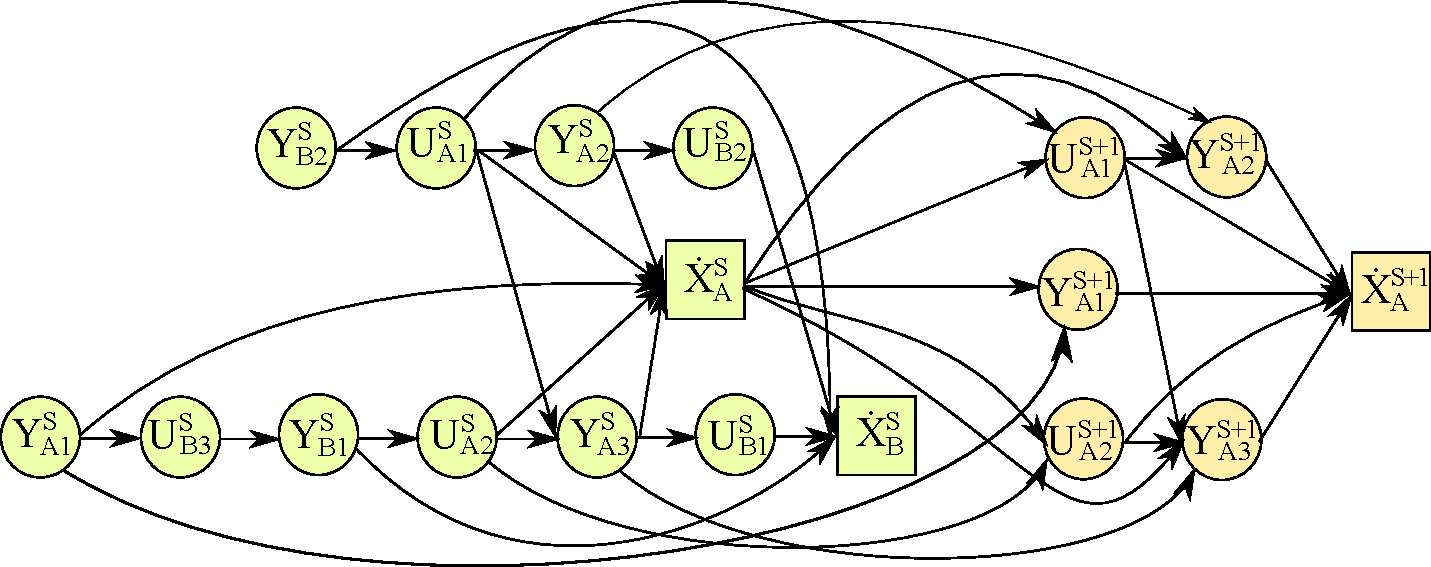
\includegraphics[scale=0.5]{figures/Operation_Graph_Two_Models_Multirate}
\caption{Graph obtained by applying the multi-rate transformation algorithm on the graph of Figure~\ref{fig:dag}}
\label{fig:dagmr}
\end{figure}

\section{Dependence Graph with Mutual Exclusion Constraints}
The FMI standard states that \textit{``FMI functions of one instance don't need to be thread safe''}. Therefore, an FMU does not implement any service to support concurrent access to its functions from multiple threads, and it is up to the executing environment to ensure the calling sequences of functions are respected as specified in the FMI standard. These restrictions introduce mutual exclusion constraints on the operations of the same FMU. We propose in this section an offline method for lightweight handling of these constraints.

\subsection{Motivation for Offline Handling of Mutual Exclusion Constraints}

In order to study the impact of mutual exclusion constraints, we have evaluated the performance obtained using two mutual exclusion strategies. The first one uses a dedicated lock (system object that guarantees mutual exclusion) for each FMU: every time an FMU function call is made at runtime, the associated lock has to be acquired before the execution of the function code can be started. The second solution is explained in \cite{benkhaled:2014} and consists in allocating the operations of a same FMU to the same core (constrained allocation). The scheduling heuristic that was used in these tests is presented in chapter \ref{ch:5-sched}. The theoretical speed-up was estimated by computing the makespan of the graph. Results are given in Figure \ref{fig:theoretical-speedup}. It shows that the expected speed-up in the case of constrained allocation is less than the one using unconstrained allocation, when the number of cores is less than five, but similar when five cores or more are available. When using less than five cores, the large number of $update_{output}$ operations can be efficiently allocated only if the unconstrained allocation is used: the speed-up difference between the constrained and unconstrained allocation cases is due to this restriction on the allocation. Five is the minimal number of cores for enabling the execution of each $update_{state}$ operation on a different core. Due to the predominant execution times of the $update_{state}$ operations, their impact on the speed-up overrides the possibility of optimizing the allocation of the other operations. This explains why the speed-up difference between the unconstrained and the constrained allocation cases becomes very small with five cores or more.

\begin{figure}[phbt]
\centering
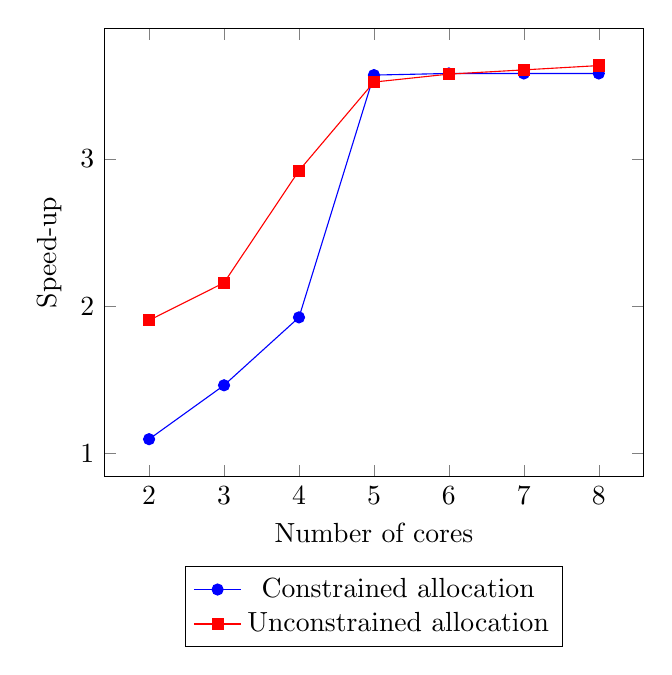
\begin{tikzpicture}
    \begin{axis}[
        xlabel=Number of cores,
        ylabel=Speed-up,legend style={at={(0.5,-0.2)},anchor=north}]
    \addplot[mark=*,blue,label=const] plot coordinates {
        (2,     1.097909998)
        (3,    1.463604418)
        (4,    1.924422442)
        (5,   3.568543452)
        (6,   3.579496624)
        (7,   3.579496624)
        (8,  3.579496624)
    };
    \addlegendentry{Constrained allocation}

    \addplot[color=red,mark=square*,label=unconst]
        plot coordinates {
        (2,     1.904310908)
        (3,    2.15962963)
        (4,   2.91987982)
        (5,   3.521135266)
        (6,  3.575107296)
        (7,  3.603831891)
        (8,  3.633021807)
        }; 
    \addlegendentry{Unconstrained allocation}
    \end{axis}
\end{tikzpicture}
\caption{Theoretical speed-up.}
\label{fig:theoretical-speedup}
\end{figure}

We implemented and tested both mutual exclusion strategies in order to compare their runtime performance. Tests were performed using the industrial use case described in chapter \ref{ch:6-eval}. Execution times measurements were performed by getting the system time stamp at the beginning of the execution and after $30$ seconds of the simulated time. As previously, we compared the speed-up by dividing the mono-core co-simulation execution time by the co-simulation execution time on a fixed number of cores. Figure \ref{fig:real-speedup} sums up the results, where unconstrained allocation corresponds to the use of lock objects. It shows the impact of mutex overhead on the speed-up. Whatever the number of the available cores, the speed-up remains close to $1.3$. On the contrary, the implementation of the constrained allocation gives similar results in terms of speed-up improvement when increasing the number of cores until five. Nevertheless, the maximum measured speed-up ($2.4$) remains smaller than the theoretical one ($3.5$). In fact, the theoretical speed-up computation considers the makespan ratio without any estimation of the runtime overhead which certainly has an important impact on the speed-up.


\begin{figure}[phbt]
\centering
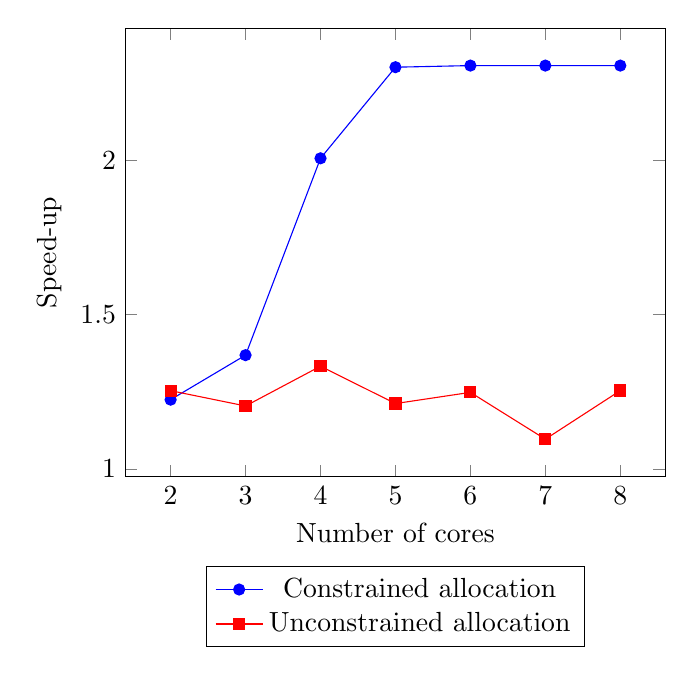
\begin{tikzpicture}
    \begin{axis}[
        xlabel=Number of cores,
        ylabel=Speed-up,legend style={at={(0.5,-0.2)},anchor=north}]
    \addplot[mark=*,blue,label=const] plot coordinates {
        (2,     1.223967163)
        (3,    1.368187328)
        (4,    2.005976773)
        (5,   2.301174325)
        (6,   2.306397786)
        (7,   2.306397786)
        (8,  2.306397786)
    };
    \addlegendentry{Constrained allocation}

    \addplot[color=red,mark=square*,label=unconst]
        plot coordinates {
        (2,     1.253126949)
        (3,    1.203511837)
        (4,   1.332430943)
        (5,   1.211351319)
        (6,  1.247650948)
        (7,  1.095957175)
        (8,  1.253420685)
        }; 
    \addlegendentry{Unconstrained allocation}
    \end{axis}
\end{tikzpicture}
\caption{Measured speed-up.}
\label{fig:real-speedup}
\end{figure}

%The obtained results show the importance of employing a mutual exclusion strategy that is efficient with regards to the limitations of allocating the operations and the introduced synchronization overhead. In the rest of this section, we attempt to attain this objective.

The restrictions introduced by employing the tested mutual exclusion techniques makes it highly desirable to find an alternative solution that could satisfy the mutual exclusion constraints while: \begin{inlinelist} \item leaving as much flexibility as possible for allocating the operations to the cores and; \item introducing lower synchronization overhead \end{inlinelist}. In the rest of this section, we suggest a method for offline handling of mutual exclusion constraints. The proposed method is based on modeling the mutual exclusion constraints in the dependence graph of the co-simulation.

\subsection{Acyclic Orientation of Mixed Graphs}

The dependence graph model can be extended in order to represent scheduling problems that involve precedence constraints and mutual exclusion constraints. This is commonly done using \textit{mixed graphs}. A mixed graph $G(V,A,D)$ is a graph which contains a set $A$ of directed arcs denoted $(o_i,o_j): 0 \leq i, j < n$ and a set $D$ of undirected edges denoted $[o_i,o_j]: 0 \leq i, j < n$. In the scheduling literature, these graphs are known as disjunctive graphs also. In addition to the precedence constraints represented by arcs as described in section \ref{sec:4-depgrph}, mutual exclusion relations are represented by edges in a mixed graph such that: 
\begin{itemize}
\item \textit{Precedence constraints:} $\forall (o_i,o_j) \in A, o_i$ must finish its execution before $o_j$ can start its execution.  
\item \textit{Mutual exclusion constraints:} $\forall [o_i,o_j] \in D, o_i$ and $o_j$ must be executed in strictly disjoint time intervals.
\end{itemize}

Operations that are connected by an edge can be executed in either order but not in parallel. In order to compute a schedule for a mixed graph, an execution order has to be defined for each pair of operations connected by an edge which is interpreted by assigning a direction to this edge. Cycles must not be introduced in the graph while assigning directions to edges, otherwise, the scheduling problem becomes infeasible. Since the final goal is to accelerate the execution of the co-simulation, and in other words, minimize the makespan of the execution of the dependence graph, the acyclic orientation of the mixed graph has to minimize the length of the critical path of the graph.

%\subsubsection{Graph Coloring of Undirected Graphs}
% Talk about Gallai–Hasse–Roy–Vitaver theorem
The acyclic orientation problem is closely related to vertex coloring. In its general form, i.e. when all edges of the graph are undirected, vertex coloring is a function $\alpha: V \rightarrow \{1, 2, \ldots, k\}$ which labels the vertices of the graph with integers, called colors, such that the inequality \ref{eq:color1} holds.

\begin{equation}
\forall\ [o_i,o_j] \in D,\ \alpha(o_i) \neq \alpha(o_j)
\label{eq:color1}
\end{equation}

The acyclic orientation of the graph can then be obtained by assigning a direction to every edge such that the color of the corresponding head vertex is smaller than the color of the corresponding tail vertex. A graph coloring with $k$ colors is referred to as \textit{k-coloring}. In its general form, vertex coloring aims at finding a \textit{minimum vertex coloring}, i.e. minimizing $k$ the number of the used colors. The minimum number of colors required to color an undirected graph is called the chromatic number and is denoted $\chi(G)$. The Gallai–Hasse–Roy–Vitaver theorem \cite{gallai:1968,roy:1967,hasse:1966,vitaver:1962} links the length of the longest path in orientations of the graph to vertex coloring of the graph. It states that the length of the longest path of a directed graph is at least $\chi(G)$. Thus, a minimum vertex coloring leads to an acyclic orientation that minimizes the length of the critical path of the resulting graph. Computing the chromatic number of a graph is NP-complete.

The acyclic orientation of a mixed graph can be obtained similarly. However, vertex coloring of a mixed graph has to take into account both arcs and edges of the graph. More precisely, a vertex coloring of a mixed graph is a function $\alpha: V \rightarrow \{1, 2, \ldots, k\}$ such that inequalities \ref{eq:color1} and \ref{eq:color2} hold.

\begin{equation}
\forall\ (o_i,o_j) \in A,\ \alpha(o_i) < \alpha(o_j)
\label{eq:color2}
\end{equation}

A coloring of a mixed graph $G(V,A,D)$ exists only if it is cycle-free \cite{ries:2007}, i.e. the induced directed graph $G(V,A,\emptyset)$ does not contain any cycle. The problem of acyclic orientation of mixed graphs has been studied in the literature in \cite{andreev:2000,sotskov:2002,al-anzi:2006}. Efficient algorithms have been proposed for special types of graphs, however in the general case it has been shown that the problem is NP-Hard.

\subsection{Problem Formulation}

In order to represent mutual exclusion constraints between FMU operations, the initial dependence graph $G(V,A)$ is transformed into a mixed graph by connecting each pair of mutually exclusive operations $o_i, o_j$ by and edge $[o_i, o_j]$. The resulting mixed graph is denoted $G(V,A,D)$ , where $V$ is the set of operations, $A$ is the set of arcs, and $D$ is the set of edges.
Once the mixed graph is constructed, directions have to be assigned to its edge in order define an order of execution for mutually exclusive operations. This transformation of the dependence graph does not impact the timing attributes of the operations. The timing constraints represented by the mixed graph $G(V,A,D)$ are given by expressions \ref{eq:color4} and \ref{eq:color5}. If operations $o_i$ and $o_j$ are connected by an arc $(o_i,o_j)$, the time interval $(S(o_i), E(o_i)]$ must precede the time interval $(S(o_j), E(o_j)]$. On the other hand, if operations $o_i$ and $o_j$ are connected by an edge $[o_i,o_j)]$, time intervals $(S(o_i), E(o_i)]$ and $(S(o_j), E(o_j)]$ must be strictly disjoint.

\begin{equation}
\forall\ (o_i,o_j) \in A,\ S(o_j) \leq \alpha(o_j)
\label{eq:color4}
\end{equation}

\begin{equation}
\forall\ [o_i,o_j] \in D,\  (S(o_i), E(o_i)] \cap (S(o_j), E(o_j)] = \emptyset
\label{eq:color5}
\end{equation}

It should be noted that, for a given edge $[o_i, o_j]$, choosing either of the execution orders does not impact the numerical results of the co-simulation since these operations do not have data dependencies. Still, we have to ensure mutual exclusion between them due to the non-thread-safe implementation of FMI. 


The problem can be stated as an optimization formulation as follows:

\begin{table}[h]
\centering
\begin{tabular}{l  l}
	
  \textit{Input} & Mixed dependence graph of operations $G_X(V_X,A_X,D_X)$\\
	\rule{0pt}{5ex}									  
	
  \textit{Output} & DAG $G_F(V_F,A_F)$\\
	\rule{0pt}{5ex}									  
  
	\textit{Find} & Assignment of colors $cr_i$ to vertices $o_i$, $\alpha: V \rightarrow \mathbb{N}$\\
	\rule{0pt}{5ex}									 
	
	\textit{Minimize} & Critical path of graph $G_F(V_F,A_F): P = max(E(o_i))_{o_i \in V}$\\
	\rule{0pt}{5ex}									 
	
	\textit{Subject to} & No cycle generated in $G_F(V_F,A_F)$\\
										 
\end{tabular}
\end{table}

\subsection{Resolution using Linear Programming}

We present here an ILP formulation for solving the problem of acyclic orientation of mixed graphs. We express the problem as a graph coloring problem where the operations can have different execution times. 

\subsubsection{Variables and Constants}

Tables \ref{table:varilporient} and \ref{table:consilporient} summarize the variables and the constants that are used respectively.

\begin{table}[!htbp]
\caption{Variables used in the ILP formulation of acyclic orientation of mixed graphs}
\centering
\label{table:varilporient}
\begin{tabular}{c c}
\toprule
Variable & Type   \\
\midrule
 $x(o_i)$ & Integer \\
 $y_{ij}$ & Binary \\
 $S(o_i)$ & Integer \\
 $E(o_i)$ & Integer \\
\bottomrule
\end{tabular}
\end{table}

\begin{table}[!htbp]
\caption{Constants used in the ILP formulation of acyclic orientation of mixed graphs}
\centering
\label{table:consilporient}
\begin{tabular}{c c}
\toprule
Constant & Type \\
\midrule
 $C(o_i)$ & Integer \\
 $M$ & Integer \\
\bottomrule
\end{tabular}
\end{table}

\subsubsection{Constraints}

We define an integer variable $x(o_i)$, which represents the color that is assigned to operation $o_i$. The inequality \ref{orient:const_1} expresses the constraint that every operations must be assigned a color that is greater than the colors of all its predecessors.

\begin{equation}
x(o_i) > x(o_j): \forall (o_j,o_i) \in A
\label{orient:const_1}
\end{equation}

The binary variable $y_{ij}$ is associated with the edge $[o_i,o_j]$ and indicates whether operation $o_i$ is assigned a color greater than the color assigned to $o_j$ or not, i.e. $y_{ij} = 1\ if x(o_i) > x(o_j), 0\ otherwise$. Note that $y_{ij}$ is the complement of $y_{ji}$. For every edge $[o_i,o_j] \in E$, the colors assigned to $o_i$ and $o_j$ must be different. Expressions \ref{orient:const_2} and \ref{orient:const_3} capture this constraint. $M$ is a big constant.

\begin{equation}
x(o_i) > x(o_j) - M \times (1-y_{ij}) + 1: \forall [o_i,o_j] \in E
\label{orient:const_2}
\end{equation} 

\begin{equation}
x(o_j) > x(o_i) - M \times y_{ij} + 1: \forall [o_i,o_j] \in E
\label{orient:const_3}
\end{equation}

Next, we need to express the computations of the timing parameters of the operations, i.e. start and end times. Recall that for a given edge $[o_i,o_j]$, if $o_j$ is assigned a color greater than the color assigned to $o_i$, then the edge $[o_i, o_j]$ is assigned a direction form $o_i$ to $o_j$. Expressions \ref{orient:const_4} and \ref{orient:const_5} are used to compute the start time of each operation and expression \ref{orient:const_6} is used to compute the end time of each operation.

\begin{equation}
S(o_i) \geq E(o_j): \forall (o_j,o_i) \in A
\label{orient:const_4}
\end{equation} 

\begin{equation}
S(o_i) \geq E(o_j) - M \times (1-y_{ij}): \forall [o_i,o_j] \in E
\label{orient:const_5}
\end{equation}

\begin{equation}
E(o_i) = S(o_i) + C(o_i): \forall o_i \in V
\label{orient:const_6}
\end{equation}
 
The critical path $P$ is computed using the inequality \ref{orient:const_7}

\begin{equation}
P \geq E(o_i): \forall o_i \in V
\label{orient:const_7}
\end{equation}

\subsubsection{Objective}

The objective of this linear program is to minimize the critical path of the dependence graph.

\begin{equation}
min(P)
\label{orient:obj}
\end{equation}


\subsection{Acyclic Orientation Heuristic}

We describe in this section a heuristic for handling mutual exclusion constraints between operations belonging to the same FMU. Without loss of generality, the superscript which denotes the number of the occurrence of an operation is not used in this section for the sake of clarity. Each vertex of the graph $G_M(V_M,A_M)$ represents an operation that we refer to using the notation $o_i$.

This mixed graph is obtained from the graph $G_M(V_M,A_M)$ by adding edges between operations belonging to the same FMU. Note that $V_X = V_M$. The orientation of the edges of $D_X$ means applying a function $\alpha :  \{[o_i,o_j] \in D_X\} \rightarrow \{(o_i,o_j),(o_j,o_i)\}$. Without loss of generality, consider that $\alpha([o_i,o_j]) = (o_i,o_j)$, then $o_i$ is added to $pred(o_j)$ and $o_j$ is added to $succ(o_i)$. Consequently, the inequality $E(o_i) \leq S(o_j)$ holds and therefore $o_i$ and $o_j$ are executed in disjoint time intervals. The first step of the heuristic consists in building the mixed graph $G_X(V_X,A_X,D_X)$ by adding edges between operations belonging to the same FMU. The output of the heuristic is a topological ordering of the operations of each FMU. This can be interpreted for each FMU $\mathcal{M}$ as an assignment of integers $\phi : V_F \rightarrow \{1,2, \dots ,m\}$ defining the order of execution for these operations, where $m$ is the number of operations of the FMU $\mathcal{M}$. We call the integer assigned to an operation its rank.

Algorithm \ref{algo:ao} details the acyclic orientation heuristic. After adding the edges to the graph, the heuristic iteratively assigns ranks to the operations. It keeps a list of already ordered operations $l$ for each FMU $\mathcal{M}$ and at each main iteration it selects the operation which has the earliest start time $S(o_i)$ to be added to the list of its FMU. Ties are broken by selecting the operation with the least flexibility $F(o_i)$. We call the operation to be ordered at a given iteration, the pending operation. The the pending operation $o_i$ is assigned the ranks $\tau \in \{x,x+1, \dots ,length(l)+1\}$ in ascending order, where \mbox{$x = \max_{o_j \in pred(o_i)}(\phi(o_j)+1)\; (1 \; if \; pred(o_i) = \emptyset)$}. For each rank $\tau$, the assignment $\phi(o_i)=\tau$ is made and the ranks assigned to all the already ordered operations $o_{i'} \in l$ such that $\phi(o_{i'}) \geq \phi(o_{i})$ are increased $\phi(o_{i'}) = \phi(o_{i'})+1$. Then, every edge $[o_i,o_i'] \in D_X : o_i' \in l$ is assigned a direction from the operation with the lower rank to the operation with the higher rank. At this point, the increase in $R$, the critical path of the graph, is evaluated. Next, the operations $o_{i'} \in l$ such that $\phi(o_{i'}) > \phi(o_{i})$ are reassigned their previous ranks $\phi(o_{i'}) = \phi(o_{i'})-1$, and the pending operation is assigned the next rank $\phi(o_i)=\phi(o_i)+1$. The increase in the critical path is evaluated again similarly. After repeating this for all the ranks $\tau \in \{x,x+1, \dots ,length(l)+1\}$, the pending operation is finally ordered at the rank which leads to the least increase in the critical path and edges $[o_i,o_i'] \in D_X : o_i' \in l$ are assigned directions as described before. The heuristic begins another iteration by selecting a new operation to be ordered. The heuristic assigns a rank to one operation at each iteration. Every operation is assigned a rank higher than the ranks of all its predecessors which guarantees that no cycle is generated. The heuristic finally stops when all the operations have been assigned ranks.

\begin{algorithm}[htb]		
	  %Initialization\;
		\textbf{Input:} Operation graph $G_M(V_M,A_M)$\;
		\textbf{Output:} New operation graph $G_F(V_F,A_F)$\;
		Set $G_M(V_M,A_M)$ the operation graph, $G_X(V_X,A_X,D_X)$ the mixed graph, and $G_F(V_F,A_F)$ the final graph\;
		$V_X \leftarrow V_M$; $A_X \leftarrow A_M$; $D_X \leftarrow \emptyset$; $V_F \leftarrow V_M$; $A_F \leftarrow A_M$\;
		Set $\Omega$ the set of all the operations: $\Omega \leftarrow V_X$\;  
 		\lForEach{pair $o_i, o_j$ such that $M(o_i) = M(o_j)$}
		{
				Add the edge $[o_i,o_j]$ to $D_X$: $D_X \leftarrow D_X \cup \{[o_i,o_j]\}$
		}
		\While{$\Omega \neq \emptyset$}
		{
			Select the operation $o_i \in \Omega$ whose start time $S(o_i) = \max_{o_j \in \Omega}(S(o_j))$. Break ties by selecting the operation with the least flexibility\;
			Set $\mathcal{M} \leftarrow M(o_i)$ and $l$ the list of the already ordered operations of FMU $\mathcal{M}$\;
			Set $\sigma \leftarrow \infty$; (Initialize the increase in the critical path)\;
			Set $x = \max_{o_j \in pred(o_i)}(\phi(o_j)+1)\; (1 \; if \; pred(o_i) = \emptyset)$\;
			\For{$\tau=x$ to $length(l) + 1$}
			{
				$\phi(o_i)=\tau$\;
				\lForEach{$o_{i'} \in l$ such that $\phi(o_{i'}) \geq \phi(o_i)$}
				{
					$\phi(o_{i'}) \leftarrow \phi(o_{i'}) + 1$
				}
				\ForEach{$o_{i'} \in l$}
				{
					\lIf{$\phi(o_{i'}) > \phi(o_i)$}
					{
						Assign a direction to the edge $[o_i,o_{i'}] \in D_X: \alpha([o_i,o_{i'}]) \leftarrow (o_i,o_{i'})$
					}
					\lElse
					{
						Assign a direction to the edge $[o_i,o_{i'}] \in D_X: \alpha([o_i,o_{i'}]) \leftarrow (o_{i'},o_i)$
					}
				}
				
				Compute the new critical path and set $\sigma'$ the increase in the critical path\;
				\lIf{$\sigma' < \sigma$}
				{
					$rank \leftarrow \tau$,
					$\sigma \leftarrow \sigma'$
				}
				\lForEach{$o_{i'} \in l$ such that $\phi(o_{i'}) > \phi(o_i)$}
				{
					Reassign $o_{i'}$ its previous rank: $\phi(o_{i'}) \leftarrow \phi(o_{i'})-1$
				}
			}
			$\phi(o_i)=rank$\;
			\ForEach{$o_{i'} \in l$}
			{
				\lIf{$\phi(o_{i'}) > \phi(o_i)$}
				{
					Assign a direction to the edge $[o_i,o_{i'}] \in D_X: \alpha([o_i,o_{i'}])\leftarrow (o_i,o_{i'})$
				}
				\lElse
				{
					Assign a direction to the edge $[o_i,o_{i'}] \in D_X: \alpha([o_i,o_{i'}])\leftarrow (o_{i'},o_i)$
				}
			}
			Remove $o_i$ from $\Omega$\;
		}
	\caption{Acyclic orientation heuristic}
	\label{algo:ao}
\end{algorithm}

\subsubsection{Complexity}

\subsubsection{Soundness}

\subsubsection{Completeness}

\subsubsection{Termination}

\section{Dependence Graph with Real-time Constraints}




